\documentclass{boi2014-lt}

\usepackage{enumitem}

\renewcommand{\DayNum}{2}
\renewcommand{\TaskCode}{portals}
\renewcommand{\TaskName}{Portalai}

\newcommand{\constant}[1]{{\tt #1}}

\begin{document}
    \begin{wrapfigure}[3]{r}{4cm}
        \vspace{-24pt}
		\includegraphics[width=4cm]{\TaskCode.jpeg}
	\end{wrapfigure}

    Kažkur labirinte paslėptas pyragas ir jūs desperatiškai norite jį suvalgyti.
    Šio labirinto žemėlapis yra lentelė sudaryta iš $R$ eilučių ir $C$ stulpelių.
    Kiekviename langelyje yra po vieną iš ženklų:
    \begin{description}[itemindent=1pt]
    	\item[\constant{\#}] (grotelės) žymi labirinto sieną,
        \item[\constant{.}] (taškas) žymi atvirą langelį,
        \item[\constant{S}] (didžioji raidė s) žymi atvirą langelį su jūsų
            dabartine pozicija,
        \item[\constant{C}] (didžioji raidė c) žymi atvirą langelį, kuriame yra
            pyragas.
    \end{description}

    Jūs galite vaikščioti tiktai atvirais langeliais ir pereiti į gretimus
    atvirus langelius, jeigu jie liečiasi kraštinėmis. Papildomai, žemėlapyje
    pavaizduota stačiakampė sritis yra atskirta nuo išorės sienomis be tarpų.
    %\todo{kurios nėra pavaizduotos žemėlapyje}.

    Tam, kad greičiau pasiektumėte pyragą, jūs įsigijote portalsvaidį iš
    Aperture Science\texttrademark{}. Bet kuriuo laiko momentu juo galite sviesti
    portalą viena iš krypčių: \emph{aukštyn}, \emph{kairėn}, \emph{žemyn} ir
    \emph{dešinėn}. Kai portalas sviedžiamas kuria nors kryptimi, jis skrenda
    tol, kol atsitrenkia į pirmą sutiktą sieną ir ant jos išsiskleidžia.

    Vienu metu gali egzistuoti daugiausiai du portalai. Jeigu du portalai jau
    išskleisti labirinte, vienas iš jų (jūsų pasirinkimu) bus pašalintas iškart,
    kai tik portalsvydis bus panaudotas dar kartą. Portalas, sviedžiamas ant
    sienos, kur jau yra išskleistas kitas portalas, pakeis ten išskleistą
    (t.y. ant kiekvienos sienos pusės daugiausiai gali būti tik vienas portalas).
    Atkreipkite dėmesį, kad keletas portalų gali būti išskleisti ant tos pačios
    sienos, bet iš kelių skirtingų pusių.

    Kai labirinte išskleisti du portalai, juos galima naudoti teleportacijai:
    jeigu stovite langelyje šalia portalo, galite į jį įeiti ir atsidurti šalia
    kito portalo. Šis veiksmas užtrunka lygiai tiek pat, kiek ir pereiti tarp
    gretimų langelių.

    Laikykite, kad portalų svaidymas neužima laiko, o perėjimas tarp gretimų
    langelių (ir teleportacija tarp portalų) užtrunka vieną laiko vienetą.

    \Task
    Duotam labirinto žemėlapiui su pažymėtomis jūsų ir pyrago pozicijomis
    apskaičiuokite trumpiausia laiką, per kurį galite pasiekti pyragą.

    \Input
    Pirmoje eilutėje yra du sveikieji skaičiai: eilučių $R$ ir stulpelių $C$
    skaičius žemėlapyje. Toliau $R$ eilučių apibūdina žemėlapį. Kiekvienoje
    eilutėje yra lygiai $C$ ženklų: \constant{\#}, \constant{.}, \constant{S}
    arba \constant{C} (kurių reikšmės buvo apibrėžtos aukščiau).

    Garantuojama, kad ženklai \constant{S} ir \constant{C} žemėlapyje bus
    panaudoti tik po vieną kartą.

    \Output
    Jūsų programa turi išvesti vieną sveikąjį skaičių -- kiek mažiausiai laiko
    vienetų užtrunka pasiekti pyragą iš pradinės pozicijos.

    Laikykite, kad iš jūsų pradinės pozicijos visada galima pasiekti pyragą.

    \Example
    \example
    {
        4 4\newline
        .\#.C\newline
        .\#.\#\newline
        ....\newline
        S...
    }
    {
        4
    }
    {
        Vienas greičiausias būdas pasiekti pyragą yra: 1) paeikite į dešinę,
        2) paeikite į dešinę, svieskite portalą į viršų ir dar vieną į apačią,
        3) įeikite į portalą žemyn -- jūs atsirasite pozicijoje ($eilutė = 0,
        stulpelis = 2$, 4) paeikite į dešinę ir čiupkite pyragą.
        
        \begin{center}
            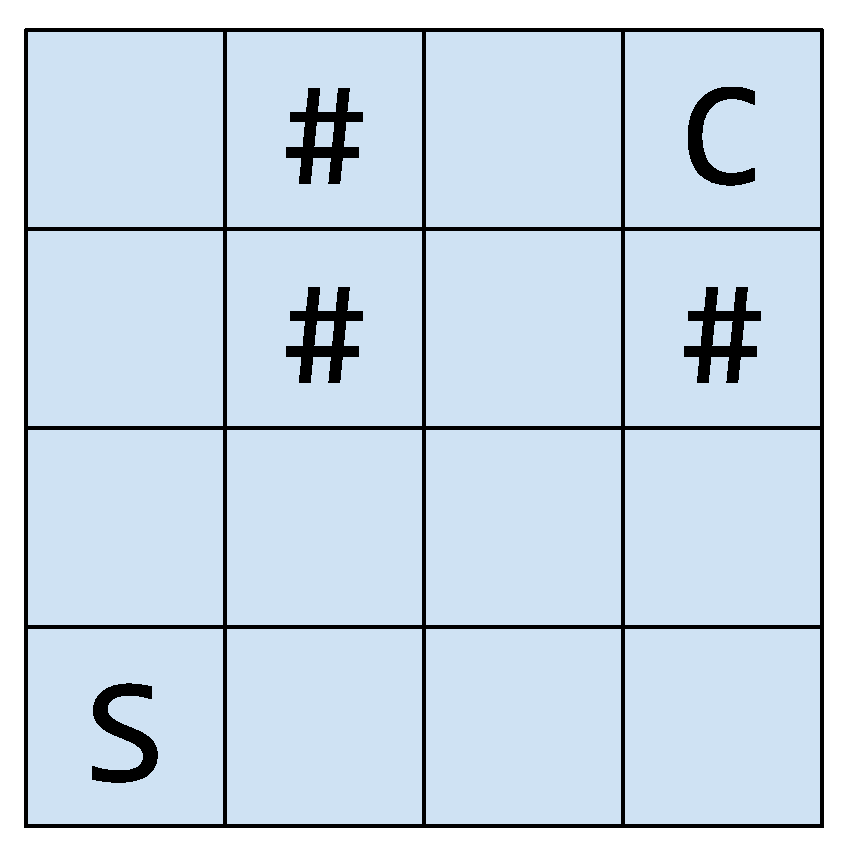
\includegraphics[width=4cm]{portals-example}
        \end{center}
    }

    \Scoring

    \begin{description}[leftmargin=0pt]
        \item[Dalinė užduotis nr. 1 (? taškų):]
            $0 \le R \le 10, 0 \le C \le 10$.
        \item[Dalinė užduotis nr. 2 (? taškų):]
            $0 \le R \le 50, 0 \le C \le 50$.
        \item[Dalinė užduotis nr. 3 (? taškų):]
            $0 \le R \le 200, 0 \le C \le 200$.
            Kiekvienas atviras langelis turi bent vieną jam gretimą sieną.
        \item[Dalinė užduotis nr. 4 (? taškų):]
            $0 \le R \le 200, 0 \le C \le 200$.
        \item[Dalinė užduotis nr. 5 (? taškų):]
            $0 \le R \le 1\ 000, 0 \le C \le 1\ 000$.
    \end{description}

    \Constraints

    \begin{description}
        \item[Laiko limitas:] ? s.
        \item[Atminties limitas:] ? MB.
    \end{description}
\end{document}
